% Packages
% sudo tlmgr install silence appendixnumberbeamer fira fontaxes mwe noto csquotes babel helvet
%--- Preamble ---------------------------------------------------------%
% Load LaTeX packages
\documentclass[aspectratio=169]{beamer}                    % supports floating text in any location
%\usetheme[noto, showmaxslides, darkmode]{pureminimalistic}
\usetheme[noto, showmaxslides, lightmode]{pureminimalistic}
\graphicspath{{logos/}}

\usepackage[utf8]{inputenc}
\usepackage{csquotes,xpatch}% recommended
%\usepackage[english]{babel}
\usepackage[american]{babel}
\babelprovide[import, main]{english}
\usepackage{tikz}
\usepackage{hyphenat}
\usepackage{graphicx}
\usepackage{tabularx}
\usepackage{booktabs}
\usepackage{bookmark}

% Hyperlinks
\usepackage{hyperref}
\hypersetup{%
	colorlinks=true,
	linkbordercolor=white,
	allcolors=blue,
	pdfborderstyle={/S/U/W 1}% border style will be underline of width 1pt
}

% Math
\usepackage{amsmath}
\usepackage{amssymb}
\usepackage{wasysym}

% Algorithms
\usepackage[ruled,vlined,english]{algorithm2e}
\SetKwFor{For}{for}{}{}

% Code
\usepackage{listings}
\usepackage{lstbayes} % Stan
\lstset{
	language=R,
	moredelim=**[is][\color{blue}]{@}{@}}

% strike through text
\usepackage[normalem]{ulem}

% Plots
\usepackage{pgfplots}
\graphicspath{{logos}{images}}
\pgfplotsset{height=6cm, % only if needed
	width=12cm,
	compat=1.17,
	legend style = {fill = white, draw = black},
	contour/every contour label/.style={
			every node/.style={mapped color!50!white,fill=white}}
}
\usepackage{tikz}
\usepackage{tikzsymbols} % Metropolis Little Man
\usetikzlibrary{shapes}
\usetikzlibrary{arrows}
\usetikzlibrary{positioning}
\usetikzlibrary{calc}
\usetikzlibrary{automata} % State in Markov Chains
\usetikzlibrary{intersections}
\usetikzlibrary{backgrounds}
\usetikzlibrary{external}
\tikzsetfigurename{fig}
\tikzexternalize[prefix=tikz/]
% Sample Space subfigures
\usepackage{subfigure}
\definecolor{gray80}{gray}{0.8}
\definecolor{gray60}{gray}{0.6}
\definecolor{colorA}{rgb}{102, 255, 255}
\definecolor{colorB}{rgb}{0, 102, 255}
\usepackage{transparent}
% Multilevel Modeling
\usepackage{adjustbox}
\newcommand*{\offset}{0.025}
\definecolor{light}{RGB}{188, 188, 220}
\definecolor{mid}{RGB}{124, 124, 185}
\definecolor{dark}{RGB}{39, 39, 143}
\definecolor{highlight}{RGB}{180, 31, 180}
% Animations
\usepackage{media9}
\usepackage{multimedia}
\addmediapath{animations}

% \renewcommand{\pageword}{}
% \renewcommand{\logoheader}{\vspace{1.5em}}

% Bibliography
\usepackage[
	%    natbib=true,
	backend=biber,
	%    style=abnt,
	%    style=authoryear-comp,
	%    style=authoryear,
	%    style=ieee,
	%    style=acm,
	%    style=apalike,
	%    style=siam,
	%    style=ieeetr,
	%    style=plain,
	style=vancouver,
	doi=true,
	eprint=false,
	hyperref=true]
{biblatex}
\addbibresource{references.bib}
% biblatex
\renewcommand*{\bibfont}{\footnotesize}
% natbib
%\def\bibfont{\footnotesize}

%% this makes it possible to add backup slides, without counting them
\usepackage{appendixnumberbeamer}
\renewcommand{\appendixname}{\texorpdfstring{\translate{appendix}}{appendix}}
% logos

% footer page
\renewcommand{\pageword}{Slide}

% Math Font Default (Fira is strange)
\renewcommand\mathfamilydefault{\rmdefault}

% footnotes
\renewcommand{\thefootnote}{\roman{footnote}}

% if loaded after begin{document} a warning will appear: "pdfauthor already used"
\title[Bayesian Workshop]{Bayesian Workshop: How to use Bayesian methods in Pumas}
\author[\textcolor{pureminimalistic@text@pumasblue}{PumasAI}]{Jose Storopoli and Mohamed Tarek \texttt{\{jose.storopoli,mohamed\}@pumas.ai}}
\institute{\textcolor{pureminimalistic@text@pumasblue}{PumasAI}}
\date{\today}


%%%% Maths crap
\newtheorem{theo}{Theorem}[]
\newtheorem{defn}{Definition}[]
\newtheorem{question}{Question}[]
\newtheorem{idea}{Idea}[]
\newtheorem{property}{Property}[]


\begin{document}
%--- Title Page -------------------------------------------------------%
\maketitle

%--- Table of Contents-------------------------------------------------%
% For longer table of contents, I find it cleaner to
% use no footline.
\begin{frame}[plain, noframenumbering]{Outline}
	\tableofcontents
\end{frame}

%--- Distributions ----------------------------------------------------%

\tikzset{
	declare function={
			discreteuniform(\a,\b)=1/(\b-\a+1);%
			binomial(\n,\p)=\n!/(x!*(\n-x)!)*\p^x*(1-\p)^(\n-x);%
			poisson(\l)=(\l^x)*exp(-\l)/(x!);%
			negativebinomial(\r,\p)=((x+\r-1)!/((\r-1)!*x!))*((1-\p)^x*\p^\r);%
			continuousuniform(\a,\b)=1/(\b-\a);%
			gaussian(\m,\s)=1/(\s*sqrt(2*pi))*exp(-((x-\m)^2)/(2*\s^2));%
			lognormal(\m,\s)=1/(x*\s*sqrt(2*pi))*exp(-((ln(x)-\m)^2)/(2*\s^2));%
			exponential(\l)=\l*exp(-\l*x);%
			gamma(\z)=2.506628274631*sqrt(1/\z)+ 0.20888568*(1/\z)^(1.5)+ 0.00870357*(1/\z)^(2.5)- (174.2106599*(1/\z)^(3.5))/25920- (715.6423511*(1/\z)^(4.5))/1244160)*exp((-ln(1/\z)-1)*\z;%
			student(\n)=gamma((\n+1)/2.)/(sqrt(\n*pi)*gamma(\n/2.))*((1+(x*x)/\n)^(-(\n+1)/2.));%
			beta(\a,\b)=(x^(\a-1)*(1-x)^(\b-1)/((gamma(\a)*gamma(\b))/gamma(\a+\b));%
			binormal(\ma,\sa,\mb,\sb,\ro)=exp(-(((x-\ma)/\sa)^2+((y-\mb)/\sb)^2-(2*\ro)*((x-\ma)/\sa)*((y-\mb)/\sb))/(2*(1-\ro^2)))/(2*pi*\sa*\sb*(1-\ro^2)^0.5);%
			conditionalbinormal(\yc,\ma,\sa,\mb,\sb,\ro)=exp(-(((x-\ma)/\sa)^2+((\yc-\mb)/\sb)^2-(2*\ro)*((x-\ma)/\sa)*((\yc-\mb)/\sb))/(2*(1-\ro^2)))/(2*pi*\sa*\sb*(1-\ro^2)^0.5);%
			sumtwonormals(\ma,\sa,\wa,\mb,\sb,\wb)=(\wa*gaussian(\ma,\sa))+(\wb*gaussian(\mb,\sb));%
			normcdf(\m,\s)=1/(1 + exp(-0.07056*((x-\m)/\s)^3 - 1.5976*(x-\m)/\s));%
		}
}

%--- Files ----------------------------------------------------------%
% !TeX root = slides.tex

\section{Pumas}
\begin{frame}{What is Pumas?}
    Pumas (\textbf{P}harmace\textbf{U}tical \textbf{M}odeling \textbf{A}nd \textbf{S}imulation)
    \parencite{rackauckas2020accelerated}
    is a suite of tools to perform quantitative analytics of various kinds
    across the horizontal of pharmaceutical drug development.
    The purpose of this framework is to bring efficient implementations of
    all aspects of the analytics in this domain under one cohesive package.
\end{frame}

\begin{frame}{Pumas Features}
    Pumas 2.3 currently includes:
    \begin{vfilleditems}
        \small
        \item Non-compartmental Analysis
        \item Specification of Nonlinear Mixed Effects (NLME) Models
        \item Simulation of NLME model using differential equations or analytical solutions
        \item Deep control over the differential equation solvers for high efficiency
        \item Estimation of NLME parameters via Maximum Likelihood, Expectation Maximization and Bayesian methods
        \item Parallelization capabilities for both simulation and estimation
        \item Mixed analytical and numerical problems
        \item Simulation and estimation diagnostics for model post-processing
        \item Interactive model exploration and diagnostics tools through webapps
        \item Automated report generation for models and non-compartmental analysis
        \item Global and local sensitivity analysis routines for multi-scale models
        \item Bioequivalence analysis
        \item Optimal design of experiments
    \end{vfilleditems}
\end{frame}
%!TEX root = slides.tex

\section{Bayesian Statistics}

\subsection{Recommended References}
\begin{frame}{Bayesian Statistics - Recommended References}
	\begin{vfilleditems}
		\item \textcite{gelman2013bayesian} - Chapter 1: Probability and inference
		\item \textcite{mcelreath2020statistical} - Chapter 1: The Golem of Prague
		\item \textcite{gelman2020regression} - Chapter 3: Some basic methods in mathematics and probability
		\item \textcite{khanBayesianLearningRule2021}
		\item \textbf{Probability}:
		\begin{vfilleditems}
			\item A great textbook - \textcite{bertsekasIntroductionProbability2nd2008}
			\item Also a great textbook (skip the frequentist part)- \textcite{dekkingModernIntroductionProbability2010}
			\item Bayesian point-of-view and also a philosophical approach- \textcite{jaynesProbabilityTheoryLogic2003}
			\item Bayesian point-of-view with a simple and playful approach - \textcite{kurtBayesianStatisticsFun2019}
			\item Philosophical approach not so focused on mathematical rigor - \textcite{diaconisTenGreatIdeas2019}
		\end{vfilleditems}
	\end{vfilleditems}
\end{frame}

\subsection{What is Bayesian Statistics?}
\begin{frame}{What is Bayesian Statistics?}
	Bayesian statistics is a \textbf{data analysis approach based on Bayes' theorem}
	where available knowledge about the parameters of a statistical model
	is updated with the information of observed data.
	\parencite{gelman2013bayesian}.
	Previous knowledge is expressed as a \textbf{prior} distribution
	and combined with the observed data in the form of a \textbf{likelihood} function
	to generate a \textbf{posterior} distribution.
	The posterior can also be used to make predictions about future events.
\end{frame}

\subsubsection{What changes from Frequentist Statistics?}
\begin{frame}{What changes from Frequentist Statistics?}
	\begin{vfilleditems}
		\item \textbf{Domain knowledge}:
		\begin{vfilleditems}
			\item You can incorporate knowledge and insights from previous studies using prior distributions on parameters
		\end{vfilleditems}
		\item \textbf{Epistemic uncertainty}:
		\begin{vfilleditems}
			\item You can quantify the epistemic uncertainty in the model parameters' values
			\item Model identifiability not necessary
			\item Works for small and large sample sizes
			\item No Gaussian assumptions
		\end{vfilleditems}
		\item \textbf{Conceptually simpler and more general}:
		\begin{vfilleditems}
			\item Uses probability theory instead of \textit{ad-hoc} methods
			\item No $p$-values, $p$-hacking and \textit{ad-hoc} assumptions in hypothesis tests
		\end{vfilleditems}
	\end{vfilleditems}
\end{frame}

\begin{frame}{A little bit more formal}
	\begin{vfilleditems}
		\item Bayesian Statistics uses probabilistic statements:
		\begin{vfilleditems}
			\item one or more parameters $\theta$
			\item unobserved data $\tilde{y}$
		\end{vfilleditems}
		\item These statements are conditioned on the observed values of $y$:
		\begin{vfilleditems}
			\item $P(\theta \mid y)$
			\item $P(\tilde{y} \mid y)$
		\end{vfilleditems}
		\item We also, implicitly, condition on the observed data from
		any covariate $x$
		\item Generally, we are interested in:
		\begin{vfilleditems}
			\item expected response of a new subject to a drug,
			e.g. $\operatorname{E}[\hat{y} \mid y]$
			\item the probability of drug effect is higher than zero,
			e.g. $P(\theta > 0 \mid y) \geq 0.95$

		\end{vfilleditems}
	\end{vfilleditems}
\end{frame}

\begin{frame}{Definition of Bayesian Statistics}
	\begin{defn}[Bayesian Statistics]
		The use of Bayes theorem as the procedure to \textbf{estimate
			parameters of interest $\theta$ or unobserved data $\tilde{y}$}.
		\parencite{gelman2013bayesian}
	\end{defn}
\end{frame}

\begin{frame}{Probability Interpretations}
	\begin{vfilleditems}
		\item \textbf{Objective} - frequency in the long run for an event:
		\begin{vfilleditems}
			\item $P(\text{rain}) = \frac{\text{days that rained}}{\text{total days}}$
			\item $P(\text{me being elected president}) = 0$ (never occurred)
		\end{vfilleditems}
		\item \textbf{Subjective} - degrees of belief in an event:
		\begin{vfilleditems}
			\item $P(\text{rain}) = \text{degree of belief that will rain}$
			\item $P(\text{me being elected president}) = 10^{-10}$ (highly unlikely)
		\end{vfilleditems}
	\end{vfilleditems}
\end{frame}

\subsubsection{What is Probability?}
\begin{frame}{What is Probability?}
	\begin{defn}[Probability]
		We define $A$ is an event and $P(A)$ the probability of event $A$.
		$P(A)$ has to be between $0$ and $1$, where higher values defines
		higher probability of $A$ happening.
		$$\begin{aligned}
				P(A)   & \in \mathbb{R} \\
				P(A)   & \in [0,1]      \\
				0 \leq & P(A) \leq 1
			\end{aligned}$$
	\end{defn}
\end{frame}

\begin{frame}{Probability Axioms\footnote{\textcite{kolmogorovFoundationsTheoryProbability1933}}}
	\begin{columns}
		\begin{column}{0.8\textwidth}
			\begin{vfilleditems}
				\item \textbf{Non-negativity}: For every $A$:
				$$P(A) \geq 0$$
				\vspace{-0.65cm}
				\item \textbf{Additivity}: For every two \textit{mutually exclusive}
				$A$ and $B$:
				$$P(A \cup B) = P(A) + P(B)$$
				\vspace{-0.65cm}
				\item \textbf{Normalization}: The probability of all possible \textit{mutually exclusive} events $A_1, A_2, \dots$ must sum up to $1$:
				$$\sum_{n \in \mathbb{N}} P(A_n) = 1$$
			\end{vfilleditems}
		\end{column}
		\begin{column}{0.2\textwidth}
			\centering
			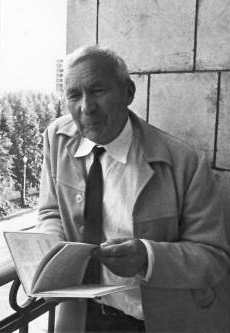
\includegraphics[width=0.9\columnwidth]{kolmogorov.jpg}
		\end{column}
	\end{columns}
\end{frame}

\begin{frame}{Sample Space\footnote{$\theta$ domain can be general, not restricted to these domains.}}
	\begin{vfilleditems}
		\item Discrete $$\Theta = \left\{1, 2, \ldots \right\}$$
		\item Continuous $$\Theta \in \left(-\infty, \infty \right)$$
	\end{vfilleditems}
\end{frame}

\begin{frame}{Discrete Sample Space}
	8 planets in our solar system:
	\begin{vfilleditems}
		\item Mercury - $\mercury$
		\item Venus - $\venus$
		\item Earth - $\earth$
		\item Mars $\mars$
		\item Jupiter - $\jupiter$
		\item Saturn $\saturn$
		\item Uranus - $\uranus$
		\item Neptune $\neptune$
	\end{vfilleditems}
\end{frame}

\begin{frame}[fragile]{Discrete Sample Space\footnote{figure adapted from \href{https://github.com/betanalpha/stan_intro}{Michael Betancourt (CC-BY-SA-4.0)}}}
	\footnotesize
	\begin{figure}
		\centering
		\subfigure{
			\begin{tikzpicture}[scale=0.25, thick]
				\draw[color=white] (-25, 0) to (10, 0);
				\node[] at (-15, 0) {The planet has a magnetic field};
				\node[] at (7, 2) {$\theta \in E_{1}$};

				\fill[color=gray60] (0, 0) circle (25pt) node[color=white] {$\mercury$};
				\fill[color=blue] (2, 0) circle (25pt) node[color=white] {$\venus$};
				\fill[color=blue] (4, 0) circle (25pt) node[color=white] {$\earth$};
				\fill[color=gray60] (6, 0) circle (25pt) node[color=white] {$\mars$};
				\fill[color=blue] (8, 0) circle (25pt) node[color=white] {$\jupiter$};
				\fill[color=blue] (10, 0) circle (25pt) node[color=white] {$\saturn$};
				\fill[color=blue] (12, 0) circle (25pt) node[color=white] {$\uranus$};
				\fill[color=blue] (14, 0) circle (25pt) node[color=white] {$\neptune$};
			\end{tikzpicture}
		}
		%
		\subfigure{
			\begin{tikzpicture}[scale=0.25, thick]
				\draw[color=white] (-25, 0) to (10, 0);
				\node[] at (-15, 0) {The planet has moon(s)};
				\node[] at (7, 2) {$\theta \in E_{2}$};

				\fill[color=gray60] (0, 0) circle (25pt) node[color=white] {$\mercury$};
				\fill[color=gray60] (2, 0) circle (25pt) node[color=white] {$\venus$};
				\fill[color=blue] (4, 0) circle (25pt) node[color=white] {$\earth$};
				\fill[color=blue] (6, 0) circle (25pt) node[color=white] {$\mars$};
				\fill[color=blue] (8, 0) circle (25pt) node[color=white] {$\jupiter$};
				\fill[color=blue] (10, 0) circle (25pt) node[color=white] {$\saturn$};
				\fill[color=blue] (12, 0) circle (25pt) node[color=white] {$\uranus$};
				\fill[color=blue] (14, 0) circle (25pt) node[color=white] {$\neptune$};
			\end{tikzpicture}
		}
		%
		\subfigure{
			\begin{tikzpicture}[scale=0.25, thick]
				\draw[color=white] (-25, 0) to (10, 0);
				\node[] at (-15, 0) {The planet has a magnetic field \textit{and} moon(s)};
				\node[] at (7, 2) {$\theta \in E_{1} \cap E_{2}$};

				\fill[color=gray60] (0, 0) circle (25pt) node[color=white] {$\mercury$};
				\fill[color=gray60] (2, 0) circle (25pt) node[color=white] {$\venus$};
				\fill[color=blue] (4, 0) circle (25pt) node[color=white] {$\earth$};
				\fill[color=gray60] (6, 0) circle (25pt) node[color=white] {$\mars$};
				\fill[color=blue] (8, 0) circle (25pt) node[color=white] {$\jupiter$};
				\fill[color=blue] (10, 0) circle (25pt) node[color=white] {$\saturn$};
				\fill[color=blue] (12, 0) circle (25pt) node[color=white] {$\uranus$};
				\fill[color=blue] (14, 0) circle (25pt) node[color=white] {$\neptune$};
			\end{tikzpicture}
		}
		%
		\subfigure{
			\begin{tikzpicture}[scale=0.25, thick]
				\node[] at (-15, 0) {The planet has a magnetic field \textit{or} moon(s)};
				\node[] at (7, 2) {$\theta \in E_{1} \cup E_{2}$};

				\fill[color=gray60] (0, 0) circle (25pt) node[color=white] {$\mercury$};
				\fill[color=blue] (2, 0) circle (25pt) node[color=white] {$\venus$};
				\fill[color=blue] (4, 0) circle (25pt) node[color=white] {$\earth$};
				\fill[color=blue] (6, 0) circle (25pt) node[color=white] {$\mars$};
				\fill[color=blue] (8, 0) circle (25pt) node[color=white] {$\jupiter$};
				\fill[color=blue] (10, 0) circle (25pt) node[color=white] {$\saturn$};
				\fill[color=blue] (12, 0) circle (25pt) node[color=white] {$\uranus$};
				\fill[color=blue] (14, 0) circle (25pt) node[color=white] {$\neptune$};
			\end{tikzpicture}
		}
		%
		\subfigure{
			\begin{tikzpicture}[scale=0.25, thick]
				\node[] at (-15, 0) {The planet does \textit{not} have a magnetic field};
				\node[] at (7, 2) {$\theta \in \neg E_{1}$};

				\fill[color=blue] (0, 0) circle (25pt) node[color=white] {$\mercury$};
				\fill[color=gray60] (2, 0) circle (25pt) node[color=white] {$\venus$};
				\fill[color=gray60] (4, 0) circle (25pt) node[color=white] {$\earth$};
				\fill[color=blue] (6, 0) circle (25pt) node[color=white] {$\mars$};
				\fill[color=gray60] (8, 0) circle (25pt) node[color=white] {$\jupiter$};
				\fill[color=gray60] (10, 0) circle (25pt) node[color=white] {$\saturn$};
				\fill[color=gray60] (12, 0) circle (25pt) node[color=white] {$\uranus$};
				\fill[color=gray60] (14, 0) circle (25pt) node[color=white] {$\neptune$};
			\end{tikzpicture}
		}
		%
	\end{figure}
\end{frame}

\begin{frame}{Continuous Sample Space\footnote{
			figure adapted from \href{https://github.com/betanalpha/stan_intro}{Michael Betancourt (CC-BY-SA-4.0)}}
	}
	\footnotesize
	\begin{figure}
		\centering
		\subfigure{
			\begin{tikzpicture}[scale=0.25, thick]
				\draw[color=white] (-27, 0) to (17, 0);
				\node[align=center] at (-15, 0) {The distance is less than five centimeters};
				\node[] at (7.5, 2) {$\theta \in E_{1}$};

				\draw[|->] (0, 0) -- (14,0) node[right] {$x$};
				\draw[line width=1mm, color=blue] (0, 0) node[] {$\,($} -- (5, 0) node[] {$\!)$};
			\end{tikzpicture}
		}
		%
		\subfigure{
			\begin{tikzpicture}[scale=0.25, thick]
				\draw[color=white] (-27, 0) to (17, 0);
				\node[align=center] at (-15, 0) {The distance is between three and seven centimeters};
				\node[] at (7.5, 2) {$\theta \in E_{2}$};

				\draw[|->] (0, 0) -- (14,0) node[right] {$x$};
				\draw[line width=1mm, color=blue] (3, 0) node[] {$\,($} -- (7,0) node[] {$\!)$};

			\end{tikzpicture}
		}
		%
		\subfigure{
			\begin{tikzpicture}[scale=0.25, thick]
				\draw[color=white] (-27, 0) to (17, 0);
				\node[align=center] at (-15, 0) {The distance is less than five centimeters \\ \textit{and} e between three and seven centimeters};
				\node[] at (7.5, 2) {$\theta \in E_{1} \cap E_{2}$};

				\draw[|->] (0, 0) -- (14,0) node[right] {$x$};
				\draw[line width=1mm, color=blue] (3, 0) node[] {$\,($} -- (5, 0) node[] {$\!)$};
			\end{tikzpicture}
		}
		%
		\subfigure{
			\begin{tikzpicture}[scale=0.25, thick]
				\draw[color=white] (-27, 0) to (17, 0);
				\node[align=center] at (-15, 0) {The distance is less than five centimeters \\ \textit{or} between three and seven centimeters};
				\node[] at (7.5, 2) {$\theta \in E_{1} \cup E_{2}$};

				\draw[|->] (0, 0) -- (14, 0) node[right] {$x$};
				\draw[line width=1mm, color=blue] (0, 0) node[] {$\,($} -- (7, 0) node[] {$\!)$};
			\end{tikzpicture}
		}
		%		%
		\subfigure{
			\begin{tikzpicture}[scale=0.25, thick]
				\draw[color=white] (-27, 0) to (17, 0);
				\node[align=center] at (-15, 0) {The distance is \textit{not} less than five centimeters};
				\node[] at (7.5, 2) {$\theta \in \neg E_{1}$};

				\draw[|->] (0, 0) -- (14, 0) node[right] {$x$};
				\draw[line width=1mm, color=blue] (5, 0) node[] {$\,($} -- (13, 0);
			\end{tikzpicture}
		}
	\end{figure}
\end{frame}

\begin{frame}{Discrete versus Continuous Parameters}
	Parameters can be continuous, such as: age, height, weight etc.
	\vfill
	All probability rules and axioms are valid also for continuous parameters.
	\vfill
	The only thing we have to do is to change all sums $\sum$ for integrals $\int$ and some probabilities $P$ with probability density (probability mass per unit measure) $p$, e.g.:
	$$\begin{aligned}
	  	p(A)         & \geq 0 \\
	  	p(A)         & \in \mathbb{R} \\
	  	\int p(A) dA & = 1
	\end{aligned}$$

\end{frame}


\begin{frame}{Conditional Probability}
	\begin{defn}[Conditional Probability]
		Probability of an event occurring in case another has occurred or not. \newline \newline
		The notation we use is $P( A \mid B )$, that read as ``the probability of
		observing $A$ given that we already observed $B$''. \newline \newline
		$$
			\begin{aligned}
				P(A \mid B) & = \frac{\text{number of elements in $A$ and $B$}}{\text{number of elements in $B$}} \\
				P(A \mid B) & = \frac{P(A \cap B)}{P(B)}
			\end{aligned}
		$$
		\newline \hspace{0.7\textwidth}
		{\footnotesize assuming that $P(B) > 0$}.
	\end{defn}
\end{frame}

\begin{frame}{Caution! Not always $P(A \mid B) = P(B \mid A)$}
	In some cases, we have the symmetry $P(A \mid K) = P(K \mid A)$,
	\textbf{but not always this is true}\footnote{
		More specific, if the basal rates $P(A)$ and $P(B)$ aren't equal,
		the symmetry is broken $P(A \mid B) \neq P(B \mid A)$}
	\begin{example}[The Pope is catholic]
		\begin{vfilleditems}
			\small{
				\item $P(\text{pope})$:
				Probability of some random person being the Pope,
				something really small, 1 in 8 billion $\left( \frac{1}{8 \cdot 10^9} \right)$
				\item $P(\text{catholic})$:
				Probability of some random person being catholic,
				1.34 billion in 8 billion $\left( \frac{1.34}{8} \approx 0.17 \right)$
				\item $P(\text{catholic} \mid \text{pope})$:
				Probability of the Pope being catholic $\left( \frac{1}{2} = 0.5 \right)$
				\item $P(\text{pope} \mid \text{catholic})$:
				Probability of a catholic person being the Pope $\left( \frac{1}{1.34 \cdot 10^9} \cdot 0.999 \approx 7.46 \cdot 10^{-10} \right)$
			}
			\item \large{\textbf{Hence}: $P(\text{catholic} \mid \text{pope}) \neq P(\text{pope} \mid \text{catholic})$}
		\end{vfilleditems}
	\end{example}
\end{frame}

\begin{frame}{Joint Probability}
	\begin{defn}[Joint Probability]
		Probability of two or more events occurring. \newline \newline
		The notation we use is $P(A, B)$, that read as
		``the probability of observing $A$ and also observing $B$''. \newline \newline
		$$
			\begin{aligned}
				P(A,B) & = \text{number of elements in $A$ or $B$} \\
				P(A,B) & = P(A \cup B)                             \\
				P(A,B) & = P(B,A)
			\end{aligned}
		$$
	\end{defn}
\end{frame}

\begin{frame}{Product Rule of Probability\footnote{also called the Product Rule of Probability.}}
	\begin{defn}[Product Rule]
		We can decompose a joint probability $P(A,B)$ into the
		product of two probabilities:
		$$
			\begin{aligned}
				P(A,B)                 & = P(B,A)                 \\
				P(A) \cdot P(B \mid A) & = P(B) \cdot P(A \mid B)
			\end{aligned}
		$$
	\end{defn}
\end{frame}

%% Bivariate Normal adapted from: https://github.com/walmes/Tikz/blob/master/src/bivariate-normal.pgf
\begin{frame}{Visualization of Joint Probability versus Conditional Probability}
	\centering
	\begin{tikzpicture}[scale=0.9]
		\begin{axis}[
				domain   = -3.5:3.5,
				domain y = -3.5:3.5,
				view = {-70}{20},
				title={$P(X,Y)$ versus $P(X \mid Y=-0.75)$},
				xlabel={$X$},
				ylabel={$Y$},
				% zlabel={$SSE(\beta_0, \beta_1)$},
				zmin = -0,
				%xticklabels=\empty,
				%yticklabels=\empty,
				zticklabels=\empty,
				xtick=\empty,
				ytick={-0.75},
				ztick=\empty,
				axis z line*=none,
				axis y line*=left,
				axis x line*= bottom]
			\addplot3 [
				domain = -3.5:3.5,
				samples = 50, samples y = 0,
				thick, smooth, color = red, fill = orange, opacity = 0.75]
			(x, -0.75, {conditionalbinormal(-0.75, 0, 1, 0, 1, 0.75)});

			\draw (-3.5, -0.75, 0) -- (3.5, -0.75, 0);

			\addplot3 [
				surf,
				domain = -3.5:3.5,
				samples = 50,
				opacity = 0.15,
				faceted color = colorB,
				colormap = {blueblack}{
						color = (colorB)
						color = (colorA!50!white)
						color = (colorA)}]
			{binormal(0, 1, 0, 1, 0.7)};
		\end{axis}
	\end{tikzpicture}
\end{frame}

%% Contour plot adapted from: https://tex.stackexchange.com/a/31713/200209
\begin{frame}{Visualization of Joint Probability versus Conditional Probability}
	\begin{columns}
		\begin{column}{0.5\textwidth}
			\centering
			\begin{tikzpicture}[scale=0.5]
				\begin{axis}[
						view={0}{90},
						axis equal,
						enlarge y limits=true,
						title={$P(X,Y)$},
						xlabel={$X$},
						ylabel={$Y$},
						xtick=\empty,
						ytick={-0.75}
					]

					\draw[red, line width=2pt] (-3.5, -0.75) -- (3.5, -0.75);

					\addplot3[contour gnuplot={labels=false},domain=-3.5:3.5,domain y=-3.5:3.5]
					{exp(-( x^2 + y^2)/3 )};

				\end{axis}
			\end{tikzpicture}
		\end{column}
		\begin{column}{0.5\textwidth}
			\centering
			\begin{tikzpicture}[scale=0.5]
				\begin{axis}[every axis plot, line width=2pt,
						title={$P(X \mid Y=-0.75)$},
						xlabel={$X$},
						ylabel={$Y$},
						xtick=\empty,
						ytick=\empty,
						domain=-3.5:3.5,samples=200,
						axis x line*=bottom,  % no box around the plot, only x and y axis
						axis y line*=left,    % the * suppresses the arrow tips
						enlarge x limits=true % extend the axes a bit
					]

					\addplot [red, fill = red, fill opacity = 0.5] {exp(-( x^2 + -0.75^2)/3 )};
				\end{axis}
			\end{tikzpicture}
		\end{column}
	\end{columns}
\end{frame}

\subsubsection{Bayes Theorem}
\begin{frame}{Who was Thomas Bayes?}
	\begin{columns}
		\begin{column}{0.8\textwidth}
			\begin{vfilleditems}
				\item \small \textbf{Thomas Bayes} (1701 - 1761) was a statistician, philosopher
				and Presbyterian minister who is known for formulating a specific
				case of the theorem that bears his name: Bayes' theorem.
				\item \small Bayes never published what would become his most famous
				accomplishment; his notes were edited and published posthumously by
				his friend \textbf{Richard Price}.
				\item \small The theorem official name is \textbf{Bayes-Price-Laplace},
				because \textbf{Bayes} was the first to discover,
				\textbf{Price} got his notes, transcribed into mathematical notation,
				and read to the Royal Society of London,
				and \textbf{Laplace} independently rediscovered the theorem without
				having previous contact in the end of the XVIII century in France
				while using probability for statistical inference with census
				data in the Napoleonic era.
			\end{vfilleditems}
		\end{column}
		\begin{column}{0.2\textwidth}
			\centering
			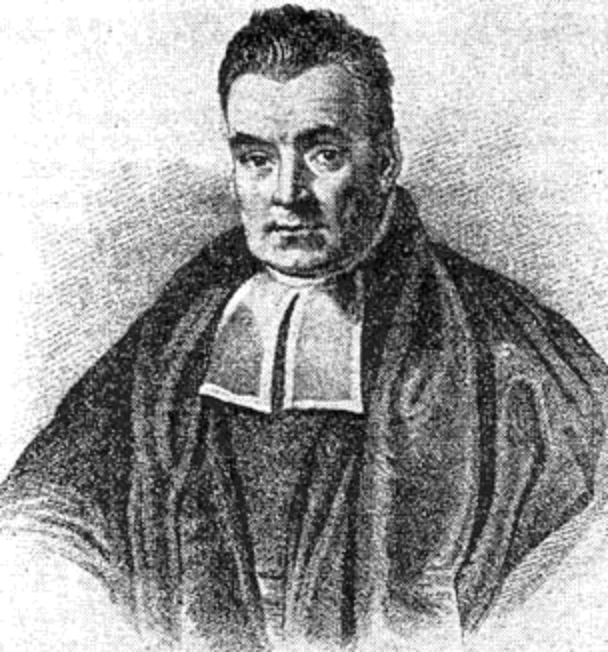
\includegraphics[width=0.9\columnwidth]{thomas_bayes.png}
		\end{column}
	\end{columns}
\end{frame}

\begin{frame}{Bayes Theorem}
	\begin{theorem}[Bayes]
		Tells us how to ``invert'' conditional probability: \newline \newline
		$$P(A \mid B) = \frac{P(A) \cdot P(B \mid A)}{P(B)}$$
	\end{theorem}
\end{frame}

\begin{frame}{Bayes' Theorem Proof}
	Remember the following probability identity:
	$$
		\begin{aligned}
			P(A,B)                 & = P(B,A)                 \\
			P(A) \cdot P(B \mid A) & = P(B) \cdot P(A \mid B)
		\end{aligned}
	$$

	OK, now divide everything by $P(B)$:
	$$
		\begin{aligned}
			\frac{P(A) \cdot P(B \mid A)}{P(B)} & = \frac{P(B) \cdot \quad P(A \mid B)}{P(B)} \\
			                                    &                                             \\
			\frac{P(A) \cdot P(B \mid A)}{P(B)} & = P(A \mid B)                               \\
			P(A \mid B)                         & = \frac{P(A) \cdot P(B \mid A)}{P(B)}
		\end{aligned}
	$$
\end{frame}

\begin{frame}{Another Probability Textbook Classic\footnote{Adapted from: \href{https://www.yudkowsky.net/rational/bayes}{Yudkowski - \textit{An Intuitive Explanation of Bayes’ Theorem}}.}}
	\begin{example}[Breast Cancer]
		\small
		How accurate is a \textbf{breast cancer} test?
		\begin{vfilleditems}
			\item \footnotesize 1\% of women have \textbf{breast cancer} (Prevalence)
			\item \footnotesize 80\% of mammograms detect \textbf{breast cancer} (True Positive)
			\item \footnotesize 9.6\% of mammograms detect \textbf{breast cancer} when there is no incidence (False Positive)
		\end{vfilleditems}
		$$
			\begin{aligned}
				P(C \mid +) & = \frac{P(+ \mid C) \cdot P(C)}{P(+)}                                                      \\
				P(C \mid +) & = \frac{P(+ \mid C) \cdot P(C)}{P(+ \mid C) \cdot P(C) + P(+ \mid \neg C) \cdot P(\neg C)} \\
				P(C \mid +) & = \frac{0.8 \cdot 0.01}{0.8 \cdot 0.01 + 0.096 \cdot 0.99}                                 \\
				P(C \mid +) & \approx 0.0776
			\end{aligned}
		$$
	\end{example}
\end{frame}


\begin{frame}{Why Bayes' Theorem is Important?}
	\begin{idea}[We can Invert the Conditional Probability]
		$$
			\begin{aligned}
				P(\text{hypothesis} \mid \text{data}) = \frac{P(\text{data} \mid \text{hypothesis}) \cdot P(\text{hypothesis})}{P(\text{data})}
			\end{aligned}
		$$
	\end{idea}
	But isn't this the $p$-value? \textcolor{red}{\textbf{NO!}}
\end{frame}

\subsection{Frequentist versus Bayesian}
\subsubsection{What are $p$-values and Confidence Intervals}
\begin{frame}{What are $p$-values?}
	\begin{defn}[$p$-value]
		$p$-value is the probability of obtaining results at least as
		extreme as the observed,
		given that the null hypothesis $H_0$ is true:
		$$P(D \mid H_0)$$
	\end{defn}
\end{frame}

\begin{frame}{What $p$-value is \textbf{not}!}
	\centering
	
\includegraphics[width=0.7\textwidth]{meme-pvalue.jpg}
\end{frame}

\begin{frame}{What $p$-value is \textbf{not}!}
	\begin{vfilleditems}
		\item \textbf{$p$-value is not the probability of the null hypothesis}
		- Infamous confusion between $P(D \mid H_0)$ and $P(H_0 \mid D)$.
		To get $P(H_0 \mid D)$ you need Bayesian statistics.
		\item \textbf{$p$-value is not the probability of data being generated at random}
		- \textcolor{red}{No!} We haven't stated nothing about randomness.
		\item \textbf{$p$-value measures the effect size of a statistical test}
		- Also \textcolor{red}{no}... $p$-value does not say anything about effect sizes.
		Just about if the observed data diverge of the expected under the null hypothesis.
		Besides, $p$-values can be hacked in several ways \parencite{head2015extent}.
	\end{vfilleditems}
\end{frame}

\begin{frame}{The relationship between $p$-value and $H_0$}
	To find out about any $p$-value, \textbf{find out what $H_0$ is behind it}.
	Its definition will never change, since it is always $P(D \mid H_0)$:
	\begin{vfilleditems}
		\item \textbf{$t$-test}: $P(D \mid \text{the difference between the groups is zero})$
		\item \textbf{ANOVA}: $P(D \mid \text{there is no difference between groups})$
		\item \textbf{Regression}: $P(D \mid \text{coefficient has a null value})$
		\item \textbf{Shapiro-Wilk}: $P(D \mid \text{population is distributed as a Normal distribution})$
	\end{vfilleditems}
\end{frame}

\begin{frame}{What are Confidence Intervals?}
	\begin{columns}
		\begin{column}{0.8\textwidth}
			\begin{defn}[Confidence Intervals]
				\begin{quotation}
					A confidence interval of X\% for a parameter is an interval
					$(a, b)$ generated by a repeated sampling procedure
					has probability X\% of containing the true value of the parameter,
					for all possible values of the parameter.
				\end{quotation}
				\vfill \vfill
				\textcite{neyman1937outline} (the ``father'' of confidence intervals)
			\end{defn}
		\end{column}
		\begin{column}{0.2\textwidth}
			\centering
			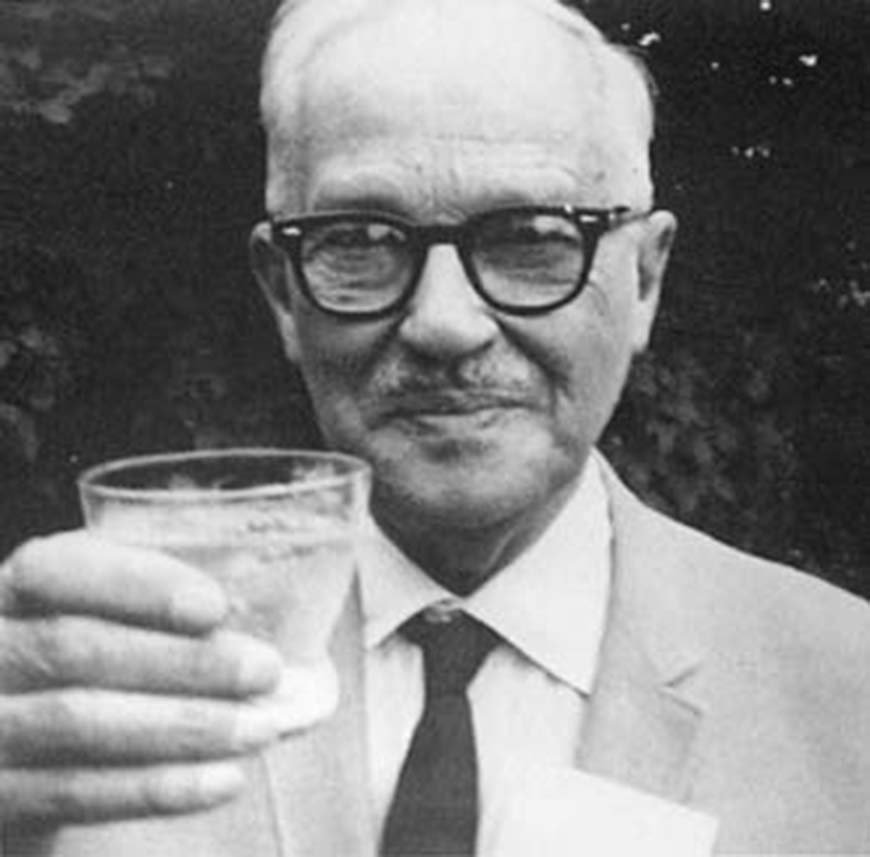
\includegraphics[width=0.9\columnwidth]{neyman.jpeg}
		\end{column}
	\end{columns}
\end{frame}

\begin{frame}{What are Confidence Intervals?}
	\begin{example}[Confidence Intervals of a Public Policy Analysis]
		Say you performed a statistical analysis to compare
		the efficacy of a public policy between two groups and you obtain a
		difference between the mean of these groups.
		You can express this difference as a confidence interval.
		Often we choose 95\% confidence.
		This means that \textbf{95 studies out of 100},
		that uses the \textbf{same sample size and target population},
		performing the \textbf{same statistical test},
		will expect to find a result of the mean difference between groups
		inside the confidence interval.
	\end{example}
	\footnotesize \textcolor{red}{Doesn't say anything about your \textbf{target population},
		but about you \textbf{sample} in an insane process of \textbf{infinite sampling} ...}
\end{frame}

\begin{frame}{Confidence Intervals versus Posterior Intervals}
	\centering
	\begin{tikzpicture}
		\begin{axis}[every axis plot, line width=2pt,
				xmin=0, xmax=4,
				ymin=0, ymax=1.5,
				ylabel=\empty,
				xlabel={$\theta$},
				samples=200,
				axis x line*=bottom, % no box around the plot, only x and y axis
				axis y line*=left,
				enlarge x limits=true, % extend the axes a bit
			]

			\addplot [blue, domain=0:4, forget plot] {lognormal(0, 2)};
			\addplot+ [
				mark=none,
				area legend,
				line width=0pt,
				color=blue,
				fill=blue, fill opacity=0.5,
				domain=0.25950495026507125:3.8534910373715427
			]
			{lognormal(0, 2)} \closedcycle;
			\addlegendentry{50\% Posterior}
			\addplot[red, mark=none] (-0.09, 1.4739034450607542) to (0.09, 1.4739034450607542);
			\addlegendentry{MLE}
			\draw [red] (0,0) to (0, 1.4739034450607542);
		\end{axis}
	\end{tikzpicture}
\end{frame}

\begin{frame}{Confidence Intervals versus Posterior Intervals}
	\centering
	\begin{tikzpicture}
		\begin{axis}[every axis plot, line width=2pt,
				xmin=-3, xmax=14,
				%ymin=0, ymax=1.5,
				ylabel=\empty,
				xlabel={$\theta$},
				samples=200,
				axis x line*=bottom, % no box around the plot, only x and y axis
				axis y line*=left,
				enlarge x limits=true, % extend the axes a bit
				%legend pos=outer north east, % there is one default value for the `legend pos' that is outside the axis
				%legend cell align=left, % so the legend looks a bit better
			]

			\addplot [blue, domain=-3:14, forget plot] {sumtwonormals(2, 1, 0.6, 10, 1, 0.4)};
			\addplot+ [
				mark=none,
				area legend,
				line width=0pt,
				color=blue,
				fill=blue, fill opacity=0.5,
				domain=1.8:9.7
			]
			{sumtwonormals(2, 1, 0.6, 10, 1, 0.4)} \closedcycle;
			\addlegendentry{50\% Posterior}
			\addplot[red, mark=none] (1.5, 0.24) to (2.5, 0.24);
			\addlegendentry{MLE}
			\draw [red] (2,0) to (2, 0.24);
		\end{axis}
	\end{tikzpicture}
\end{frame}

\begin{frame}{But why I never see stats without $p$-values?}
	\begin{columns}
		\begin{column}{0.8\textwidth}
			We cannot understand $p$-values if we do no not comprehend
			its origins and historical trajectory.
			The first mention of $p$-values was made by the statistician
			Ronald Fischer in 1925 \parencite{fisher1925statistical}:
			\begin{quotation}
				[$p$-value is a] measure of evidence against the null hypothesis
			\end{quotation}
			\begin{vfilleditems}
				\item To quantify the strength of the evidence against the null hypothesis,
				Fisher defended ``$p<0.05$ as the standard level to conclude that there is evidence against the tested hypothesis''
				\item ``We should not be off-track if we draw a conventional line at 0.05''
			\end{vfilleditems}
		\end{column}
		\begin{column}{0.2\textwidth}
			\centering
			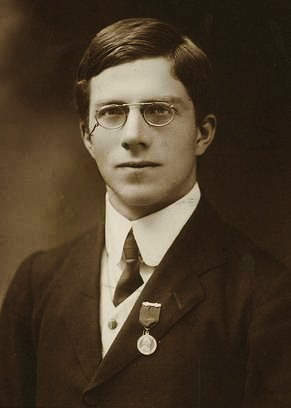
\includegraphics[width=0.9\columnwidth]{fisher.jpg}
		\end{column}
	\end{columns}
\end{frame}

\begin{frame}{$p = 0.06$}
	\begin{vfilleditems}
		\item Since $p$-value is a probability, it is also a continuous measure.
		\item There is no reason for us to differentiate $p = 0.049$ against $p = 0.051$.
		\item Robert Rosenthal, a psychologist said ``surely, God loves the $.06$ nearly as much as the $.05$''~\parencite{rosnow1989statistical}.
	\end{vfilleditems}
\end{frame}

\begin{frame}{But why I never heard about Bayesian statistics?\footnote{\textit{inverse probability}
			was how Bayes' theorem was called in the beginning of the 20th century}}
	\begin{columns}
		\begin{column}{0.8\textwidth}
			\begin{quotation}
				… it will be sufficient … to reaffirm my personal conviction …
				that the theory of inverse probability is founded upon an error,
				and must be wholly rejected.
			\end{quotation}
			\vfill \vfill
			\textcite{fisher1925statistical}
		\end{column}
		\begin{column}{0.2\textwidth}
			\centering
			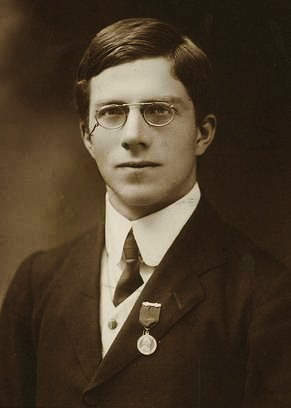
\includegraphics[width=0.9\columnwidth]{fisher.jpg}
		\end{column}
	\end{columns}
\end{frame}

\begin{frame}{Inside every non-Bayesian, there is a Bayesian struggling to get out\footnote{
			quote from Dennis Lindley}}
	\begin{columns}
		\begin{column}{0.8\textwidth}
			\begin{vfilleditems}
				\item In his final year of life,
				Fisher published a paper \parencite{fisherExamplesBayesMethod1962}
				examining the possibilities of Bayesian methods,
				but with the prior probabilities being determined experimentally.
				\item Some authors speculate \parencite{jaynesProbabilityTheoryLogic2003}
				that if Fisher were alive today, he would probably be a Bayesian.
			\end{vfilleditems}
		\end{column}
		\begin{column}{0.2\textwidth}
			\centering
			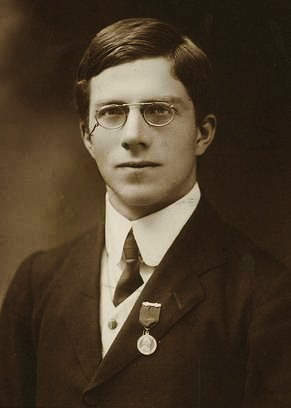
\includegraphics[width=0.9\columnwidth]{fisher.jpg}
		\end{column}
	\end{columns}
\end{frame}

\subsection{Bayesian Statistics}
\begin{frame}{Bayes' Theorem as an Inference Engine}
	\footnotesize Now that you know what is probability and Bayes' theorem,
	I will propose the following:
	$$
		\underbrace{P(\theta \mid y)}_{\text{Posterior}} = \frac{\overbrace{P(y \mid  \theta)}^{\text{Likelihood}} \cdot \overbrace{P(\theta)}^{\text{Prior}}}{\underbrace{P(y)}_{\text{Normalizing Constant}}}
	$$
	\begin{vfilleditems}
		\item \footnotesize $\theta$ -- parameter(s) of interest
		\item \footnotesize $y$ -- observed data
		\item \footnotesize \textbf{Priori}: prior probability of the parameter(s) value(s)
		\item \footnotesize \textbf{Likelihood}: probability of the observed data given the parameter(s) value(s)
		\item \footnotesize \textbf{Posterior}: posterior probability of the parameter(s) value(s) after we observed data $y$
		\item \footnotesize \textbf{Normalizing Constant}\footnote{sometimes also called \textit{evidence}.}: $P(y)$ gives a measure of the likelihood of the entire model class which is useful when considering multiple models.
		This probability is transformed and can be interpreted as something that only exists so that the result $P(y \mid \theta) P(\theta)$ be constrained between $0$ e $1$
		-- a valid probability.
	\end{vfilleditems}
\end{frame}

\begin{frame}{Bayes' Theorem as an Inference Engine}
	Bayesian statistics allows us to \textbf{quantify directly the uncertainty}
	related to the value of one or more parameters of our model given the
	observed data.
	This is the \textbf{main feature} of Bayesian statistics,
	since we are estimating directly $P(\theta \mid y)$ using Bayes' theorem.
	The resulting estimate is totally intuitive:
	simply quantifies the uncertainty that we have about the value of one or more
	parameters given the data, model assumptions (likelihood) and the prior
	probability of these parameter's values.
\end{frame}

% \subsubsection{Advantages of Bayesian Statistics}
% \begin{frame}{Bayesian vs Frequentist Stats}
% 	%\begin{table}[h!]
% 	\centering
% 	\small
% 	\begin{tabular}{|l|p{.3\textwidth}|p{.3\textwidth}|}
% 		\toprule
% 		                     & \textcolor{blue}{\textbf{Bayesian Statistics}}       & \textcolor{red}{\textbf{Frequentist Statistics}}                       \\ \midrule
% 		\textbf{Data}        & Fixed –- Non-random                                  & Uncertain –- Random                                                    \\ \midrule
% 		\textbf{Parameters}  & Uncertain –- Random                                  & Fixed –- Non-random                                                    \\ \midrule
% 		\textbf{Inference}   & Uncertainty regarding the parameter value            & Uncertainty regarding the sampling process from an infinite population \\ \midrule
% 		\textbf{Probability} & Subjective\footnote{with highly informative priors.} & Objective (but with several model assumptions)                         \\ \midrule
% 		\textbf{Uncertainty} & Posterior Interval –- $P(\theta \mid y)$             & Confidence Interval –- $P(y \mid \theta)$                              \\
% 		\bottomrule
% 	\end{tabular}
% 	%\end{table}
% \end{frame}

%!TEX root = slides.tex

\section{Priors}

\subsection{Recommended References}
\begin{frame}{Priors and Posteriors - Recommended References}
	\begin{vfilleditems}
		\item \textcite{gelman2013bayesian}:
		\begin{vfilleditems}
			\item Chapter 2: Single-parameter models
			\item Chapter 3: Introduction to multiparameter models
		\end{vfilleditems}
		\item \textcite{mcelreath2020statistical} - Chapter 4: Geocentric Models
		\item \textcite{gelman2020regression}:
		\begin{vfilleditems}
			\item Chapter 9, Section 9.3: Prior information and Bayesian synthesis
			\item Chapter 9, Section 9.5: Uniform, weakly informative, and informative priors in regression
		\end{vfilleditems}
		\item \textcite{vandeschootBayesianStatisticsModelling2021}
	\end{vfilleditems}
\end{frame}

\begin{frame}{Prior Probability }
	Bayesian statistics is characterized by the use of prior information
	as the prior probability $P(\theta)$, often just prior:
	$$
		\underbrace{P(\theta \mid y)}_{\text{Posterior}} = \frac{\overbrace{P(y \mid  \theta)}^{\text{Likelihood}} \cdot \overbrace{P(\theta)}^{\text{Prior}}}{\underbrace{P(y)}_{\text{Normalizing Constant}}}
	$$
\end{frame}

\subsection{The subjectivity of the Prior}
\begin{frame}{The subjectivity of the Prior}
	\begin{vfilleditems}
		\item Many criticisms to Bayesian statistics are due the subjectivity
		in eliciting priors probability on certain hypothesis or model parameter's values.
		\item Subjectivity is something unwanted in the ideal picture of the
		scientist and the scientific method.
	\end{vfilleditems}
	\textbf{Counter-arguments}:
	\begin{vfilleditems}
		\item Very weak priors avoid subjectivity.
		\item Anything that involves human action will never be free from
		subjectivity.
		We have subjectivity in everything and science is \textcolor{red}{no} exception.
		% \item The creative and deductive process of theory and hypotheses formulations
		% is \textbf{not} objective.
		\item Frequentist statistics is also subjective, since there is \textbf{A LOT} of subjectivity in
		choosing the model and target p-value \parencite{jaynesProbabilityTheoryLogic2003, vandeschootBayesianStatisticsModelling2021}
	\end{vfilleditems}
\end{frame}

% \begin{frame}{How to Incorporate Subjectivity}
% 	\begin{vfilleditems}
% 		\item Bayesian statistics \textbf{embraces} subjectivity while
% 		frequentist statistics \textbf{bans} it.
% 		\item For Bayesian statistics, \textbf{subjectivity guides our inferences}
% 		and leads to more robust and reliable models that can assist in
% 		decision making.
% 		\item Whereas, for frequentist statistics, \textbf{subjectivity is a taboo}
% 		and all inferences should be objective,
% 		even if it resorts to \textbf{hiding and omitting model assumptions}.
% 		\item Bayesian statistics also has assumptions and subjectivity,
% 		but these are \textbf{declared and formalized}
% 	\end{vfilleditems}
% \end{frame}

\subsection{Types of Priors}

\begin{frame}{Types of Priors}
	In general, we can have 3 main types of priors in a Bayesian approach
	\parencite{gelman2013bayesian, mcelreath2020statistical, vandeschootBayesianStatisticsModelling2021}:
	\begin{vfilleditems}
		\item \textbf{uniform (flat)}: not recommended.
		\item \textbf{weakly informative}: little domain knowledge added.
		\item \textbf{informative}: medium to high domain knowledge.
	\end{vfilleditems}
\end{frame}

% \subsubsection{Uniform Prior (Flat)}
% \begin{frame}{Uniform Prior (Flat)}
% 	Starts from the premise that ``everything is possible''.
% 	There is no limits in the degree of beliefs that the distribution of certain
% 	values must be or any sort of restrictions.
% 	\vfill
% 	Flat and super-vague priors are not usually recommended and some thought
% 	should included to have at least weakly informative priors.
% 	\vfill
% 	Formally, an uniform prior is an uniform distribution over all the
% 	possible support of the possible values:
% 	\begin{vfilleditems}
% 		\item \textbf{model parameters}: $\{\theta \in \mathbb{R} : -\infty < \theta < \infty\}$
% 		\item \textbf{model error or residuals}: $\{\sigma \in \mathbb{R}^+ : 0 \leq \theta < \infty\}$
% 	\end{vfilleditems}
% \end{frame}

\subsubsection{Prior Selection}
\begin{frame}{Prior Selection}
	\begin{center}
	\begin{tabular}{||p{0.2\linewidth} p{0.7\linewidth}||} 
	 \hline
	 Support & Distributions \\ [0.5ex] 
	 \hline\hline
	 (0, 1) & \lstinline{Beta}, \lstinline{KSOneSided}, \lstinline{NoncentralBeta}, \lstinline{LogitNormal} \\ 
	 \hline
	 $\mathcal{R}^+$ & \lstinline{BetaPrime}, \lstinline{Chi}, \lstinline{Chisq}, \lstinline{Erlang}, \lstinline{Exponential}, \lstinline{FDist}, \lstinline{Frechet}, \lstinline{Gamma}, \lstinline{InverseGamma}, \lstinline{InverseGaussian}, \lstinline{Kolmogorov}, \lstinline{LogNormal}, \lstinline{NoncentralChisq}, \lstinline{NoncentralF}, \lstinline{Rayleigh}, \lstinline{Weibull} \\
	 \hline
	 $\mathcal{R}$ & \lstinline{Cauchy}, \lstinline{Gumbel}, \lstinline{Laplace}, \lstinline{Logistic}, \lstinline{Normal}, \lstinline{NormalCanon}, \lstinline{NormalInverseGaussian}, \lstinline{PGeneralizedGaussian}, \lstinline{TDist} \\  [1ex] 
	 \hline
	\end{tabular}
	\end{center}
\end{frame}

\begin{frame}{Prior Selection}
	\begin{center}
	\begin{tabular}{||p{0.2\linewidth} p{0.7\linewidth}||} 
	 \hline
	 Support & Distributions \\ [0.5ex] 
	 \hline\hline
	 $\mathcal{R}$ vectors & \lstinline{MvNormal} \\
	 \hline
	 $\mathcal{R}^+$ vectors & \lstinline{MvLogNormal} \\
	 \hline
	 PD mats & \lstinline{Wishart}, \lstinline{InverseWishart} \\
	 \hline
	 Corr mats & \lstinline{LKJ}, \lstinline{LKJCholesky} \\
	 \hline
	 Other & \lstinline{Constrained}, \lstinline{truncated}, \lstinline{LocationScale}, \lstinline{Uniform}, \lstinline{Arcsine}, \lstinline{Biweight}, \lstinline{Cosine}, \lstinline{Epanechnikov}, \lstinline{Semicircle}, \lstinline{SymTriangularDist}, \lstinline{Triweight}, \lstinline{Pareto}, \lstinline{GeneralizedPareto}, \lstinline{GeneralizedExtremeValue}, \lstinline{Levy} \\ [1ex] 
	 \hline
	\end{tabular}
	\end{center}
\end{frame}

\begin{frame}{Prior Selection}
  \vfill
  Check \textbf{similar} models from literature. If you really have to choose a new prior, follow the following process:
  \vfill
  \begin{vfilleditems}
	 \item Decide the \textbf{support} of the prior. The support of the prior distribution must match the the domain of the parameter.
	 \item Decide the \textbf{center} of the prior, e.g. mean, median or mode.
	 \item Decide the \textbf{strength} of the prior. This is often controlled by a standard deviation or scale parameter in the distribution constructor.
	 \item Decide the \textbf{shape} of the probability density function (PDF) of the prior. Left skewed, right skewed, centered, heavy tail, etc.
  \end{vfilleditems}
\end{frame}

\begin{frame}{Prior Selection}
  A prior too strong around the wrong parameter values can negatively hurt your study.
  \vfill
  It will then require many more observations to infer a posterior distribution centered around the true data generating parameter values.
  \vfill
  A prior too weak can often hinder the performance of the inference.
\end{frame}

% \subsubsection{Weekly Informative Prior}
% \begin{frame}{Weekly Informative Prior}
% 	Here we start to have ``educated'' guess about our parameter values.
% 	Hence, we don't start from the premise that ``anything is possible''.
% 	\vfill
% 	I recommend always to transform the priors of the problem at hand into
% 	something centered in $0$ with standard deviation of $1$\footnote{
% 		this is called standardization,
% 		transforming all variables into $\mu=0$ and $\sigma=1$.}:
% 	\vfill
% 	\begin{vfilleditems}
% 		\item $\theta \sim \text{Normal}(0, 1)$ (Andrew Gelman's preferred choice\footnote{
% 			see more about prior choices in the
% 			\href{https://github.com/stan-dev/stan/wiki/Prior-Choice-Recommendations}{\texttt{Stan}'s GitHub wiki}.})
% 		\item $\theta \sim \text{Student}(\nu=3, 0, 1)$ (Aki Vehtari's preferred choice)
% 	\end{vfilleditems}
% \end{frame}

\subsubsection{Priors for Covariance Matrices}
\begin{frame}{Priors for Covariance Matrices}
	We can specify a prior for a covariance matrix
	$\boldsymbol{\Sigma}$.
	\vfill
	For computational efficiency,
	we can make the covariance matrix $\boldsymbol{\Sigma}$ into a correlation matrix.
	Every covariance matrix can be decomposed into:
	$$
		\boldsymbol{\Sigma}=\text{diag}_\text{matrix}(\boldsymbol{\tau}) \cdot \mathbf{C} \cdot \text{diag}_\text{matrix}(\boldsymbol{\tau})
	$$
	where $\mathbf{C}$ is a correlation matrix with
	$1$s in the diagonal and the off-diagonal elements between -1 and 1 $\rho \in (-1, 1)$.
	$\boldsymbol{\tau}$ is a vector composed of the variables' variances from
	$\boldsymbol{\Sigma}$ (is is the $\boldsymbol{\Sigma}$'s diagonal).
\end{frame}

\begin{frame}{Priors for Covariance Matrices}
	\small
	Additionally, the correlation matrix $\mathbf{C}$
	can be decomposed once more for greater computational efficiency.
	Since all correlations matrices are symmetric and positive definite
	(all of its eigenvalues are real numbers $\mathbb{R}$ and positive $>0$),
	we can use the \href{https://en.wikipedia.org/wiki/Cholesky_decomposition}
	{Cholesky Decomposition}
	to decompose it into a triangular matrix
	(which is much more computational efficient to handle):
	$$
		\mathbf{C} = \mathbf{L}_{\mathbf{C}} \mathbf{L}^T_{\mathbf{C}}
	$$
	where $\mathbf{L}_{\mathbf{C}}$ is a lower-triangular matrix.
	\vfill
	What we are missing is to define a prior for the correlation matrix $\mathbf{C}$.
\end{frame}

\subsubsection{Simulating from the prior}
\begin{frame}{Simulating from the prior}
It can be useful sometimes to simulate from the model propagating the uncertainty from the prior distributions to the model predictions.
\vfill
Predictions from the model can further be plotted against the observations to get a feel for the behavior of the prior model. 
\end{frame}

% \section{Probability Distributions}

\subsection{Recommended References}
\begin{frame}{Probability Distributions - Recommended References}
	\begin{vfilleditems}
		\item \textcite{grimmettProbabilityRandomProcesses2020}
		\begin{vfilleditems}
			\item Chapter 3: Discrete random variables
			\item Chapter 4: Continuous random variables
		\end{vfilleditems}
		\item \textcite{dekkingModernIntroductionProbability2010}
		\begin{vfilleditems}
			\item Chapter 4: Discrete random variables
			\item Chapter 5: Continuous random variables
		\end{vfilleditems}
		\item \textcite{betancourtProbabilisticBuildingBlocks2019}
	\end{vfilleditems}
\end{frame}

%--- Intro -----------------------------------------------------------%
\begin{frame}{Probability Distributions}
	Bayesian statistics uses probability distributions as the inference
	engine of the parameter and uncertainty estimates.
	\vfill
	Imagine that probability distributions are small ``Lego'' pieces.
	We can construct anything we want with these little pieces.
	We can make a castle, a house, a city; literally anything.
	The same is valid for Bayesian statistical models.
	We can construct models from the simplest ones to the most complex
	using probability distributions and their relationships.
\end{frame}

\begin{frame}
	\begin{defn}[Probability Distribution Function]
		A probability distribution function is a mathematical function
		that outputs the probabilities for different results of an
		experiment.
		It is a mathematical description of a random phenomena in terms
		of its sample space and the event probabilities (subsets
		of the sample space).
		$$P(X): X \to \mathbb{R} \in [0, 1]$$
		For discrete random variables, we define as ``mass'',
		and for continuous random variables, we define as ``density''.
	\end{defn}
\end{frame}

\begin{frame}{Mathematical Notation}
	We use the notation
	$$X \sim \text{Dist}(\theta_1, \theta_2, \dots)$$
	where:
	\begin{vfilleditems}
		\item $X$: random variable
		\item Dist: distribution name
		\item $\theta_1, \theta_2, \dots$: parameters that define how the
		distribution behaves
	\end{vfilleditems}
	Every probability distribution can be ``parameterized'' by specifying
	parameters that allow to control certain distribution aspects for
	a specific goal.
\end{frame}

\begin{frame}{Probability Distribution Function}
	\centering
	\begin{tikzpicture}
		\begin{axis}[every axis plot, line width=2pt,
				ylabel=PDF,
				xlabel={$X$},
				domain=-4:4,samples=200,
				axis x line*=bottom, % no box around the plot, only x and y axis
				axis y line*=left, % the * suppresses the arrow tips
				enlarge x limits=true, % extend the axes a bit
			]

			\addplot [blue] {gaussian(0, 1)};
		\end{axis}
	\end{tikzpicture}
\end{frame}

\begin{frame}
	\begin{defn}[Cumulative Distribution Function]
		The cumulative distribution function (CDF) of a random variable
		$X$ evaluated at $x$ is the probability that $X$ will take
		values less or qual than $x$:
		$$\text{CDF} = P(X \leq x)$$
	\end{defn}
\end{frame}

\begin{frame}{Cumulative Distribution Function}
	\centering
	\begin{tikzpicture}
		\begin{axis}[every axis plot, line width=2pt,
				ylabel=CDF,
				xlabel={$X$},
				domain=-4:4,samples=200,
				axis x line*=bottom, % no box around the plot, only x and y axis
				axis y line*=left, % the * suppresses the arrow tips
				enlarge x limits=true, % extend the axes a bit
			]

			\addplot [blue] {normcdf(0, 1)};
		\end{axis}
	\end{tikzpicture}
\end{frame}

%--- Discrete --------------------------------------------------------%
\subsection{Discrete Distributions}
\begin{frame}
	\begin{defn}[Discrete Distributions]
		Discrete probability distributions are distributions which the
		results are a discrete number:
		$-N, \dots, -2, 1, 0,1,2,\dots, N$ e $N \in \mathbb{Z}$.
		In discrete probability distributions we call the probability
		of a distribution taking certain values as ``mass''.
		The probability mass function (PMF) is the function that
		specifies the probability of a random variable $X$ taking value $x$:
		$$\text{PMF}(x) = P(X = x)$$
	\end{defn}
\end{frame}

\subsubsection{Discrete Uniform}
\begin{frame}{Discrete Uniform}
	The discrete uniform is a symmetric probability distribution in which
	a finite number of values are equally likely of being observable.
	Each one of the $n$ values have probability $\frac{1}{n}$.
	\vfill
	The uniform discrete distribution has two parameters and its notation is
	$\text{Uniform}(a, b)$:
	\begin{vfilleditems}
		\item $a$ -- lower bound
		\item $b$ -- upper bound
	\end{vfilleditems}
	\vfill
	Example: dice.
\end{frame}

\begin{frame}{Discrete Uniform}
	$$\text{Uniform}(a,b) = f(x, a, b) = \frac{1}{b-a+1} \text{ for $a \leq x \leq b$ and $x\in \{a,a+1,\dots ,b-1,b\}$}$$
\end{frame}

\begin{frame}{Discrete Uniform}
	\centering
	\begin{tikzpicture}
		\begin{axis}[every axis plot,
				ybar=0pt, bar width=0.3,
				ylabel=PMF,
				samples at={1,...,6}, % All plots: from 1:6, 6 samples only
				axis x line*=bottom, % no box around the plot, only x and y axis
				axis y line*=left, % the * suppresses the arrow tips
				enlarge x limits=true, % extend the axes a bit
			]

			\addplot [fill=blue] {discreteuniform(1, 6)};
			\addlegendentry{$a=1, b=6$}
		\end{axis}
	\end{tikzpicture}
\end{frame}

\subsubsection{Bernoulli}
\begin{frame}{Bernoulli}
	Bernoulli distribution describes a binary event of the success of an experiment.
	We represent $0$ as failure and $1$ as success, hence the result of a
	Bernoulli distribution is a binary variable $Y \in \{0, 1\}$.
	\vfill
	Bernoulli distribution is often used to model binary discrete results
	where there is only two possible results.
	\vfill
	Bernoulli distribution has only a single parameter and its notation is
	$\text{Bernoulli} (p)$:
	\begin{vfilleditems}
		\item $p$ -- probability of success
	\end{vfilleditems}
	\vfill
	Example: If the patient survived or died or if the client purchased or not.
\end{frame}

\begin{frame}{Bernoulli}
	$$\text{Bernoulli}(p) = f(x, p)=p^{x}(1-p)^{1-x} \text{ for $x \in \{0,1\}$}$$ %
\end{frame}

\begin{frame}{Bernoulli}
	\centering
	\begin{tikzpicture}
		\begin{axis}[every axis plot,
				ybar=0pt, bar width=0.5,
				ymin=0,
				xmin=-0.25, xmax=1.25,
				ylabel=PMF,
				axis x line*=bottom, % no box around the plot, only x and y axis
				axis y line*=left, % the * suppresses the arrow tips
				enlarge x limits=true, % extend the axes a bit
				xtick={0, 1}
			]

			\addplot [fill=blue] coordinates {
					(0, 0.6)
					(1, 0.4)};
			\addlegendentry{$p=\frac{1}{3}$}
		\end{axis}
	\end{tikzpicture}
\end{frame}

\subsubsection{Binomial}
\begin{frame}{Binomial}
	The binomial distribution describes an event in which the number of
	successes in a sequence $n$ independent experiments,
	each one making a yes--no question with probability of success $p$.
	Notice that Bernoulli distribution is a special case of the binomial
	distribution where $n=1$.
	\vfill
	The binomial distribution has two parameters and its notation is
	$\text{Binomial}(n, p)$ :
	\begin{vfilleditems}
		\item $n$ -- number of experiments
		\item $p$ -- probability of success
	\end{vfilleditems}
	\vfill
	Example: number of heads in five coin throws.
\end{frame}

\begin{frame}{Binomial}
	$$\text{Binomial}(n,p) = f(x, n, p) = \binom{n}{x}p^{x}(1-p)^{n-x} \text{ for $x \in \{0, 1, \dots, n\}$}$$
\end{frame}

\begin{frame}{Binomial}
	\centering
	\begin{tikzpicture}
		\begin{axis}[every axis plot,
				ybar=0pt, bar width=1,
				ylabel=PMF,
				ytick={0,0.05,...,0.15},
				samples at={0,...,40},
				axis x line*=bottom, % no box around the plot, only x and y axis
				axis y line*=left, % the * suppresses the arrow tips
				enlarge x limits=true, % extend the axes a bit
				y tick label style={/pgf/number format/.cd, fixed, fixed zerofill, precision=2}
			]

			\addplot [fill=blue, fill opacity=0.5] {binomial(40, 0.2)};
			\addlegendentry{$n=40, p=\frac{1}{5}$}
			\addplot [fill=red, fill opacity=0.5] {binomial(40, 0.5)};
			\addlegendentry{$n=40, p=\frac{1}{2}$}
		\end{axis}
	\end{tikzpicture}
\end{frame}

\subsubsection{Poisson}
\begin{frame}{Poisson}
	Poisson distribution describes the probability of a certain number of
	events occurring in a fixed time interval if these events
	occur with a constant mean rate which is known and independent since
	the time of last occurrence.
	Poisson distribution can also be used for number of events in other
	type of intervals, such as distance, area or volume.
	\vfill
	Poisson distribution has one parameter and its notation is $\text{Poisson}(\lambda)$:
	\begin{vfilleditems}
		\item $\lambda$ -- rate
	\end{vfilleditems}
	\vfill
	Example: number of e-mails that you receive daily or the number of the potholes you'll find in your commute.
\end{frame}

\begin{frame}{Poisson}
	$$\text{Poisson}(\lambda) = f(x, \lambda) = \frac{\lambda^x e^{-\lambda}}{x!} \text{ for $\lambda > 0$}$$
\end{frame}

\begin{frame}{Poisson}
	\centering
	\begin{tikzpicture}
		\begin{axis}[every axis plot,
				ybar=0pt, bar width=1,
				ylabel=PMF,
				samples at={0,...,8},
				axis x line*=bottom, % no box around the plot, only x and y axis
				axis y line*=left, % the * suppresses the arrow tips
				enlarge x limits=true, % extend the axes a bit
			]

			\addplot [fill=blue, fill opacity=0.5] {poisson(1)};
			\addlegendentry{$\lambda=2$}
			\addplot [fill=red, fill opacity=0.5] {poisson(4)};
			\addlegendentry{$\lambda=4$}
		\end{axis}
	\end{tikzpicture}
\end{frame}

\subsubsection{Negative Binomial}
\begin{frame}{Negative Binomial\footnote{
			any phenomena that can be modeles as a Poisson distribution can be
			modeled also as negative binomial distribution
			\parencite{gelman2013bayesian, gelman2020regression}.}}
	\small
	The binomial distribution describes an event in which the number of
	successes in a sequence $n$ independent experiments,
	each one making a yes--no question with probability of success $p$
	until $k$ successes.
	Notice that it becomes the Poisson distribution in the limit as $k \to \infty$.
	This makes it a robust option to replace a Poisson distribution to model
	phenomena with overdispersion
	(presence of greater variability in data than would be expected).
	\vfill \small
	The negative binomial has two parameters and its notation is
	$\text{Negative Binomial}(k, p)$:
	\begin{vfilleditems}
		\small
		\item $k$ -- number of successes
		\item $p$ -- probability of success
	\end{vfilleditems}
	\vfil \small
	Example: annual occurrence of tropical cyclones.
\end{frame}

\begin{frame}{Negative Binomial}
	$$
		\begin{aligned}
			\text{Negative Binomial}(k, p) & = f(x, k, p) & = \binom{x + k - 1}{k - 1}p^{x}(1-p)^{k} \\
			\\
			                               & ~            & \text{for $x \in \{0, 1, \dots, n\}$}
		\end{aligned}
	$$
\end{frame}

\begin{frame}{Negative Binomial}
	\centering
	\begin{tikzpicture}
		\begin{axis}[every axis plot,
				ybar=0pt, bar width=1,
				ylabel=PMF,
				samples at={0,...,8},
				axis x line*=bottom, % no box around the plot, only x and y axis
				axis y line*=left, % the * suppresses the arrow tips
				enlarge x limits=true, % extend the axes a bit
			]

			\addplot [fill=blue, fill opacity=0.5] {negativebinomial(1, 0.5)};
			\addlegendentry{$k=1, p=\frac{1}{2}$}
			\addplot [fill=red, fill opacity=0.5] {negativebinomial(5,0.5)};
			\addlegendentry{$k=5, p=\frac{1}{2}$}
		\end{axis}
	\end{tikzpicture}
\end{frame}

%--- Continuous ------------------------------------------------------%

\subsection{Continuous Distributions}
\begin{frame}
	\begin{defn}[Continuous Distributions]
		\small
		Continuous probability distributions are distributions which
		the results are values in a continuous real number line:
		$(-\infty, +\infty) \in \mathbb{R}$.
		In continuous probability distributions we call the probability
		of a distribution taking values as ``density''.
		Since we are referring to real numbers we cannot obtain the
		probability of a random variable $X$ taking exactly the value $x$.
		This will always be $0$, since we cannot specify the exact
		value of $x$. $x$ lies in the real number line, hence,
		we need to specify the probability of $X$ taking values in an
		interval $[a,b]$.
		The probability density function (PDF) is defined as:
		$$\text{PDF}(x) = P(a \leq X \leq b) = \int_a^b f(x) dx$$
	\end{defn}
\end{frame}

\subsubsection{Continuous Uniform}
\begin{frame}{Continuous Uniform}
	The continuous uniform distribution is a symmetric probability distribution
	in which an infinite number of value intervals are equally likely of being observable.
	Each one of the infinite $n$ intervals have probability $\frac{1}{n}$.
	\vfill
	The continuous uniform distribution has two parameters and its notation is $\text{Uniform}(a, b)$:
	\begin{vfilleditems}
		\item $a$ -- lower bound
		\item $b$ -- upper bound
	\end{vfilleditems}
\end{frame}

\begin{frame}{Continuous Uniform}
	$$\text{Uniform}(a,b) = f(x, a, b) = \frac{1}{b-a} \text{ for $a \leq x \leq b$ e $x \in [a, b]$}$$
\end{frame}

\begin{frame}{Continuous Uniform}
	\centering
	\begin{tikzpicture}
		\begin{axis}[every axis plot, line width=2pt,
				ylabel=PDF,
				domain=0:6,samples=200,
				axis x line*=bottom, % no box around the plot, only x and y axis
				axis y line*=left, % the * suppresses the arrow tips
				enlarge x limits=true, % extend the axes a bit
			]

			\addplot [blue] {continuousuniform(0, 6)};
			\addlegendentry{$a=0, b=6$}
		\end{axis}
	\end{tikzpicture}
\end{frame}

\subsubsection{Normal}
\begin{frame}{Normal}
	This distribution is generally used in social and natural sciences to
	represent continuous variables in which its underlying distribution are unknown.
	This assumption is due to the central limit theorem (CLT) that,
	under precise conditions, the mean of many samples (observations) of a
	random variable with finite mean and variance is itself a random variable
	which the underlying distribution converges to a normal distribution
	as the number of samples increases (as $n \to \infty$).
	\vfill
	Hence, physical quantities that we assume that are the sum of many
	independent processes (with measurement error) often have underlying
	distributions that are similar to normal distributions.
\end{frame}

\begin{frame}{Normal}
	The normal distribution has two parameters and its notation is
	$\text{Normal}(\mu, \sigma^2)$ or $\text{N}(\mu, \sigma^2)$:
	\begin{vfilleditems}
		\item $\mu$ -- mean of the distribution, and also median and mode
		\item $\sigma$ -- standard deviation\footnote{sometimes is also parameterized as variance $\sigma^2$.},
		a dispersion measure of how observations occur in relation from the mean
	\end{vfilleditems}
	\vfill
	Example: height, weight etc.
\end{frame}

\begin{frame}{Normal\footnote{
			see how the normal distribution was derived from the binomial
			distribution in the \hyperlink{appendixnormal}{backup slides}.}}
	$$\text{Normal}(\mu,\sigma) = f(x, \mu, \sigma) = \frac{1}{\sigma{\sqrt{2\pi }}}e^{-{\frac{1}{2}}\left({\frac {x-\mu }{\sigma }}\right)^{2}} \text{ for $\sigma > 0$}$$
\end{frame}

\begin{frame}{Normal}
	\centering
	\begin{tikzpicture}
		\begin{axis}[every axis plot, line width=2pt,
				ylabel=PDF,
				domain=-4:6,samples=200,
				axis x line*=bottom, % no box around the plot, only x and y axis
				axis y line*=left, % the * suppresses the arrow tips
				enlarge x limits=true, % extend the axes a bit
			]

			\addplot [blue] {gaussian(0, 1)};
			\addlegendentry{$\mu=0, \sigma=1$}
			\addplot [red] {gaussian(0, 2)};
			\addlegendentry{$\mu=0, \sigma=2$}
			\addplot [yellow] {gaussian(2, 1)};
			\addlegendentry{$\mu=2, \sigma=1$}
		\end{axis}
	\end{tikzpicture}
\end{frame}

\subsubsection{Log-Normal}
\begin{frame}{Log-Normal}
	The log-normal distribution is a continuous probability distribution of a
	random variable which its natural logarithm is distributed as a normal distribution.
	Thus, if the natural logarithm a random variable $X$, $\ln(X)$, is distributed
	as a normal distribution, then $Y = \ln(X)$ is normally distributed and
	$X$ is log-normally distributed.
	\vfill
	A a log-normal random variable only takes positive real values.
	It is a convenient and useful model for measurements in exact and engineering
	sciences, as well as in biomedical, economical and other sciences.
	For example, energy, concentrations, length, financial returns and other measurements.
	\vfill
	A log-normal process is the statistical realization of a multiplicative
	product of many independent positive random variables.
\end{frame}

\begin{frame}{Log-Normal}
	The log-normal distribution has two parameters and its notation is
	$\text{Log-Normal}(\mu, \sigma^2)$:
	\begin{vfilleditems}
		\item $\mu$ -- mean of the distribution's natural logarithm
		\item $\sigma$ -- square root of the variance of the distribution's natural logarithm
	\end{vfilleditems}
\end{frame}

\begin{frame}{Log-Normal}
	$$\text{Log-Normal}(\mu,\sigma) = f(x, \mu, \sigma) = \frac{1}{x \sigma{\sqrt{2\pi}}}e^{-\left({\frac {(\ln(x)-\mu)^2}{2 \sigma^2 }}\right)} \text{ for $\sigma > 0$}$$
\end{frame}

\begin{frame}{Log-Normal}
	\centering
	\begin{tikzpicture}
		\begin{axis}[every axis plot, line width=2pt,
				ylabel=PDF,
				domain=0:5,samples=200,
				axis x line*=bottom, % no box around the plot, only x and y axis
				axis y line*=left, % the * suppresses the arrow tips
				enlarge x limits=true, % extend the axes a bit
			]

			\addplot [blue] {lognormal(0, 0.25)};
			\addlegendentry{$\mu=0, \sigma=\frac{1}{4}$}
			\addplot [red] {lognormal(0, 1)};
			\addlegendentry{$\mu=0, \sigma=1$}
			\addplot [yellow] {lognormal(1, 1)};
			\addlegendentry{$\mu=1, \sigma=1$}
		\end{axis}
	\end{tikzpicture}
\end{frame}

\subsubsection{Exponential}
\begin{frame}{Exponential}
	The exponential distribution is the probability distribution of the time
	between events that occurs in a continuos manner, are independent,
	and have constant mean rate of occurrence.
	\vfill
	The exponential distribution has one parameter and its notation is
	$\text{Exponential}(\lambda)$:
	\begin{vfilleditems}
		\item $\lambda$ -- rate
	\end{vfilleditems}
	\vfill
	Example: How long until the next earthquake or how long until the next bus arrives.
\end{frame}

\begin{frame}{Exponential}
	$$\text{Exp}(\lambda) = f(x, \lambda) = \lambda e^{-\lambda x} \text{ for $\lambda > 0$}$$
\end{frame}

\begin{frame}{Exponential}
	\centering
	\begin{tikzpicture}
		\begin{axis}[every axis plot, line width=2pt,
				ylabel=PDF,
				domain=0:5,samples=200,
				axis x line*=bottom, % no box around the plot, only x and y axis
				axis y line*=left, % the * suppresses the arrow tips
				enlarge x limits=true, % extend the axes a bit
			]

			\addplot [blue] {exponential(0.5)};
			\addlegendentry{$\lambda=\frac{1}{2}$}
			\addplot [red] {exponential(1)};
			\addlegendentry{$\lambda=1$}
			\addplot [yellow] {exponential(2)};
			\addlegendentry{$\lambda=2$}
		\end{axis}
	\end{tikzpicture}
\end{frame}

\subsubsection{Student's $t$}
\begin{frame}{Student's $t$}
	Student's $t$ distribution arises by estimating the mean of a normally-distributed
	population in situations where the sample size is small and the standard
	deviation is known\footnote{this is where the ubiquitous Student's $t$ test.}.
	\vfill
	If we take a sample of $n$ observations from a normal distribution,
	then Student's $t$ distribution with $\nu = n-1$ degrees of freedom can
	be defined as the distribution of the location of the sample mean
	in relation to the true mean, divided by the sample's standard deviation,
	after multiplying by the scaling term $\sqrt{n}$.
	\vfill
	Student's $t$ distribution is symmetric and in a bell-shape,
	like the normal distribution, but with long tails,
	which means that has more chance to produce values far away from its mean.
\end{frame}

\begin{frame}{Student's $t$}
	Student's $t$ distribution has one parameter and its notation is
	$\text{Student}(\nu)$:
	\begin{vfilleditems}
		\item $\nu$ -- degrees of freedom, controls how much it resembles a normal distribution
	\end{vfilleditems}
	\vfill
	Example: a dataset full of outliers.
\end{frame}

\begin{frame}{Student's $t$}
	$$\text{Student}(\nu) = f(x, \nu) = \frac{\Gamma \left(\frac{\nu+1}{2} \right)} {\sqrt{\nu\pi}\,\Gamma \left(\frac{\nu}{2} \right)} \left(1+\frac{x^2}{\nu} \right)^{-\frac{\nu+1}{2}} \text{ for $\nu \geq 1$}$$
\end{frame}

\begin{frame}{Student's $t$}
	\centering
	\begin{tikzpicture}
		\begin{axis}[every axis plot, line width=2pt,
				ylabel=PDF,
				domain=-4:4,samples=200,
				axis x line*=bottom, % no box around the plot, only x and y axis
				axis y line*=left, % the * suppresses the arrow tips
				enlarge x limits=true, % extend the axes a bit
			]

			\addplot [blue] {student(1)};
			\addlegendentry{$\nu=1$}
			\addplot [red] {student(3)};
			\addlegendentry{$\nu=3$}
			\addplot [yellow] {student(30)};
			\addlegendentry{$\nu=30$}
		\end{axis}
	\end{tikzpicture}
\end{frame}

\subsubsection{Beta}
\begin{frame}{Beta}
	The beta distribution is a natural choice to model anything that is
	restricted to values between $0$ e $1$.
	Hence, it is a good candidate to model probabilities and proportions.
	\vfill
	The beta distribution has two parameters and its notations is
	$\text{Beta} (\alpha, \beta)$:
	\begin{vfilleditems}
		\item $\alpha$ or sometimes $a$ -- shape parameter,
		controls how much the shape is shifted towards $1$
		\item $\beta$ or sometimes $b$ -- shape parameter,
		controls how much the shape is shifted towards $0$
	\end{vfilleditems}
	\vfill
	Example: A basketball player that has already scored 5 free throws and
	missed 3 in a total of 8 attempts -- $\text{Beta}(3, 5)$
\end{frame}

\begin{frame}{Beta}
	$$\text{Beta} (\alpha, \beta) = f(x, \alpha, \beta) \frac{x^{\alpha-1}(1-x)^{\beta-1}} {\frac{\Gamma (\alpha )\Gamma (\beta )}{\Gamma (\alpha +\beta )}} \text{ for $\alpha,\beta > 0$ and $x \in [0, 1]$}$$
\end{frame}

\begin{frame}{Beta}
	\centering
	\begin{tikzpicture}
		\begin{axis}[every axis plot, line width=2pt,
				ylabel=PDF,
				domain=0:1,samples=200,
				axis x line*=bottom, % no box around the plot, only x and y axis
				axis y line*=left, % the * suppresses the arrow tips
				enlarge x limits=true, % extend the axes a bit
			]

			\addplot [blue] {beta(1,1)};
			\addlegendentry{$\alpha=\beta=1$}
			\addplot [red] {beta(3,2)};
			\addlegendentry{$\alpha=3,\beta=2$}
			\addplot [yellow] {beta(2,3)};
			\addlegendentry{$\alpha=2,\beta=3$}
		\end{axis}
	\end{tikzpicture}
\end{frame}


\section{References}
\begin{frame}[allowframebreaks, noframenumbering]{References}
	\printbibliography
\end{frame}

\appendix % do not count the following slides for the total number
\section*{Backup Slides}
\begin{frame}[plain, noframenumbering]
	\centering
	\vfill
	{\fontsize{40}{50}\selectfont Backup Slides}
	\vfill
\end{frame}

\end{document}
